\chapter{PolyStep Edit Page:}
The PolyStep Edit page is used to program sequences for the Analog 4 or attached External MIDI device.

% \screenshot{}
\encodersbuttons{Trig Condition}{MicroTiming}{Track Length}{--}{Toggle Ext/MD}{PageSelect}{Rotate View}{Track/Trig Menu}

\textit{To enter the PolyStep edit mode:\\Enter the MD Step Edit mode by pressing \textbf{[PageSelect + Trigger 5]}. Then Press the \textbf{[Save]} button to enter PolyStep Edit Page.}\\
\section{Track Selection in PolyStep edit mode:}
If using the Analog 4, select the desired track using the A4’s track select buttons. The first note played on the mini keyboard will cause the PolyStep edit page to switch to  the corresponding external sequencer track.
\section{Poly Sequencer: }
The Poly Sequencer is a ‘Note on’ and ‘Note off’ sequencer. There is no note length, instead for each ‘Note on’ event, a corresponding ‘Note off’ event should be placed on a step elsewhere in the sequence.

Each step can hold a maximum of 4 events either NoteOn or NoteOff.\\\\
\fbox{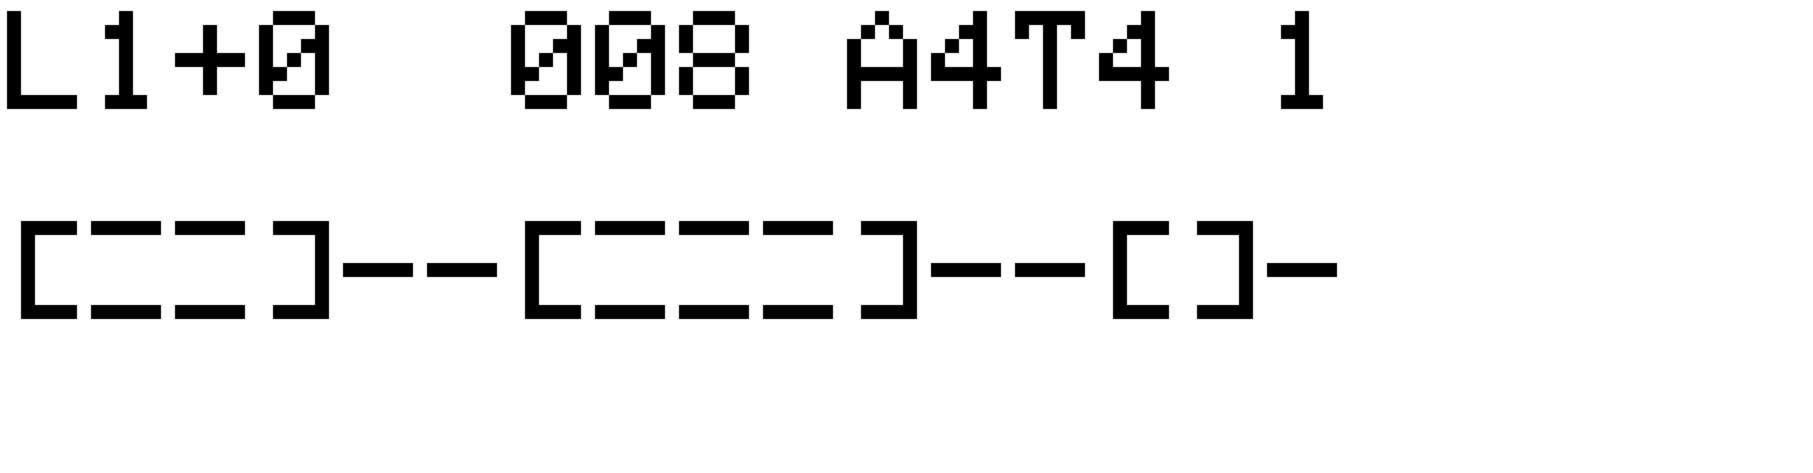
\includegraphics[scale=.40]{seq_ext_step_page.png}}\\
\\
NoteOn events notes are shown in uppercase. E.g: C 3, A\#4, B 5, D\#6
\\NoteOff events notes are shown in lowercase. E.g: c 3, a\#4, b 5, d\#6
\\\\
The first note event entered for a specific note number is always of event type NoteOn.\\
The next time the same note is entered it will automatically be placed as a NoteOff event.

\section{Program a Sequence: }
The trigger interface on the MD is used to edit the steps of the step sequence in the PolyStep Edit page.

The notes of the Analog4 keyboard or External Midi keyboard are used to edit the note data.

\begin{enumerate}
\item Press and hold the desired trigger on the MD whilst simultaneously pressing one or a maximum of 4 notes on the Analog4/Ext keyboard.
\item Adjust conditional mode or microtiming as needed using encoders 1 and 2.
\item Repeat the above for another step in the sequence, (Selecting the exact same notes). This time the notes will be entered as NoteOff events.
\end{enumerate}

\section{Clearing a sequence:}
\begin{itemize}
\item To clear the current track, press and hold the\textbf{ [ Shift2 ]} to open the track menu, rotate \textbf{[Encoder2]} to the entry \textbf{CLEAR}, then rotate \textbf{[Encoder1]} to select \textbf{TRK}.
\item To clear all MD tracks, select \textbf{ALL}
\end{itemize}

\vspace{-0.3cm}

\section{Rotating visible sequence:}
Each polyphonic track consists of 8 pages of 16 steps, for a total of 128 steps per track.
\begin{itemize}
\item Rotate the current track-page by pressing the \textbf{[Write] }button.
\end{itemize}

\vspace{-0.3cm}

\section{Changing track length:}
\begin{itemize}
\item Track length is controlled by rotating \textbf{[ Encoder 3 ]}. Only steps less than the current track length are drawn.
\item To change the lengths of all 4 polyphonic tracks simultaneously hold down \textbf{[Write]} whilst rotating \textbf{[ Encoder 3 ]}.
\item Track length can also be set by holding \textbf{[Write]} and then selecting the corresponding step from the MD trigger interface. The track length is offset by the current track-page.
\end{itemize}

\vspace{-0.3cm}

\section{Track Speed:}
All sequencer tracks can be played at various speeds. 1x, 2x, 3/2x, 4/3x, 1/2x, 1/4x, 1/8x. Triplets can be achieved using either 3/2x, 4/3x.\\

The EXT tracks perform slightly differently to the MD sequencer tracks. At 1x speed two successive notes can only be played at a minimum 32th note interval. Thus, the EXT Track should be set to 2x speed if you intend to play successive 16th notes. Ext tracks have an extended 128 step length to accommodate for this difference.

\vspace{-0.3cm}
